\documentclass[11pt,a4paper]{article}
\usepackage{acl}
\geometry{margin=1.5cm}
\usepackage{times}
\usepackage{latexsym}
\usepackage[T1]{fontenc}
\usepackage[utf8]{inputenc}
\usepackage{microtype}
\usepackage{graphicx}
\usepackage{booktabs}
\usepackage{enumitem}
\usepackage{tikz}
\usetikzlibrary{shapes.geometric, arrows.meta, positioning}

\title{MediSim: Multimodal Diagnostic and Agentic Triage System\\
Progress Report}

\author{
  \mdseries Htut Ko Ko(st126010), Imtiaz Ahmad(st126685), \\
  \mdseries Michael R. Lacar(st126161) and Aashutosh Raut(st126438) \\
  \mdseries Asian Institute of Technology
}

\begin{document}
\maketitle
\thispagestyle{plain}
\pagestyle{plain}

\begin{abstract}
Traditional digital healthcare systems struggle to process unstructured multimodal patient inputs and complex triage queries safely. We propose MediSim, a unified system featuring a Multimodal Diagnostic Assistant and a Multi-Agent Triage framework. By fusing CNN and pretrained Transformer architectures for images and text, and orchestrating role-based LLM agents for triage, we establish a self-verifying clinical pipeline. Our multimodal fusion model achieved a testing accuracy of 51.08\% and an F1-score of 46.82\% on the IU X-Ray dataset, providing a 5.04\% absolute accuracy improvement over the 46.04\% baseline ResNet model. The entire system is successfully deployed as a full-stack React and FastAPI web interface, establishing a functional, hallucination-resistant clinical pipeline.

\paragraph{Keywords:} Multimodal AI, Agentic Triage, Medical Vision-Language, Clinical Safety.
\end{abstract}

\section{Introduction}

% Paragraph 1: Background
In recent years, the integration of Artificial Intelligence into healthcare has promised to revolutionize clinical diagnostics and remote patient triage. Medical vision-language models have shown robust initial capabilities in parsing radiology scans alongside clinical reports \citep{bu2024dynamic}, while Large Language Models (LLMs) are increasingly deployed to emulate clinical reasoning in conversational formats \citep{lu2024triageagent}. These advancements theoretically allow for remote diagnostic tools that can rapidly interpret complex, unstructured patient data spanning both medical imaging and textual symptomatology.

% Paragraph 2: The Gap
However, existing diagnostic systems generally treat medical imaging and conversational triage as entirely disparate pipelines, requiring massive computational resources and exhibiting high risk for clinical hallucination when interacting with patients. While lightweight unimodal networks like CNNs and LSTMs perform symptom classification effectively \citep{mullenbach2018explainable}, they have been largely superseded by pretrained Transformer encoders that offer superior contextual understanding computationally off-the-shelf. Furthermore, they lack dynamic interaction. Conversely, end-to-end medical LLMs remain computationally dense and prone to unsafe generative behaviors in critical medical decision-making scenarios, requiring robust mitigation strategies \citep{sahu2025occutriage}. Specifically, the gap lies in the absence of a unified, lightweight system that can orchestrate standard CNN/LSTM pipelines for deterministic multimodal analysis while simultaneously operating a constrained, multi-agent LLM framework to cross-verify dynamic triage symptoms.

% Paragraph 3: Your Work
Therefore, we propose MediSim: a Multimodal Diagnostic and Agentic Triage System. MediSim comprises two selectable features. First, it processes synchronized image (Chest X-ray) and patient symptom text using an ensemble of CNN and pretrained Transformer architectures to output preliminary diagnostic reports. Second, it facilitates interactive triage through a structured Multi-Agent framework comprising specific roles, including a Triage Nurse, Specialist Doctor, and Medical Fact-Checker. Technically, the Fact-Checker explicitly grounds its verification against Longitudinal Memory and authoritative Electronic Medical Records (EMR). A failed check is rigorously defined as any recommendation presenting a physiological contraindication, prompting an immediate override of the Specialist's output with a safe fallback protocol.

% Paragraph 4: Key Findings (Anticipated for Proposal)
Our implementation phase yielded highly promising quantitative results on the 15-class diagnostic dataset. During training and evaluation on 2,771 samples from the IU X-Ray dataset, our Multimodal Fusion model established a testing accuracy of 51.08\% and an F1-Score of 46.82\%. This represented a 5.04\% absolute accuracy leap over the baseline ResNet18-only configuration (46.04\% Accuracy, 43.52\% F1). The user interface is now fully operational, displaying dynamic Model Insights metrics via hot-reloading cards mapping directly to our Jupyter training outputs.

% Paragraph 5: Significance & Contributions
Ultimately, by delivering a functional, cross-verified pipeline that operates efficiently on consumer hardware, this project holds significance for secure AI deployment in low-resource environments. The primary \textbf{contributions} of this work include:
\begin{enumerate}[noitemsep]
    \item A unified multimodal architecture matching radiology scans with patient-reported symptoms.
    \item A role-based multi-agent verification protocol to mitigate clinical hallucinations in dynamic triage.
    \item A lightweight implementation feasible for resource-constrained edge environments.
\end{enumerate}

\section{Related Work}

\paragraph{Multimodal Medical Image and Text Analysis:} 
A vital theme in recent literature is the alignment of medical imaging, such as Chest X-rays, with radiology narratives. Traditional image-captioning methods face difficulty processing long, structured narratives with subtle anomalies \citep{liu2021contrastive}. Recent approaches have mitigated this by using dynamic knowledge prompting \citep{bu2024dynamic} or learning fine-grained associations between image regions and individual sentences \citep{wang2023fine}. Despite these advances, these models are frequently isolated and focus heavily on automated reporting for clinicians rather than patient-facing multimodal symptom alignment, indicating a gap for lightweight patient-interactive fusion systems.

\paragraph{Agentic AI and LLM Triage:} 
The deployment of LLMs for clinical interaction has shifted from single-agent paradigms toward collaborative multi-agent architectures \citep{lu2024triageagent}. Single-agent chatbots are susceptible to hallucination and unsafe behavior in specialized healthcare settings \citep{sahu2025occutriage, wu2025kamac}. By implementing simulated agent networks consisting of diverse clinical roles, researchers have shown that collaborative models consistently outperform solitary models by utilizing consensus and debate mechanisms \citep{fan2025aihospital}. MediSim expands on this by grounding the multi-agent system’s context using the deterministic outputs from the preceding multimodal vision-language pipeline. 

\paragraph{Pretrained Clinical Text Classification:}
Before the dominance of heavy transformer models, attention-based CNNs and Bidirectional LSTMs successfully dominated clinical concept extraction and patient risk assessment from free text. Recent studies show that transitioning from LSTMs to pretrained Transformer embeddings achieves superior precision metrics on real-world clinical notes by leveraging broad clinical pretraining rather than learning from scratch \citep{mullenbach2018explainable, girardi2018patient}. We draw upon these established methods to build a computationally accessible baseline for interpreting patient symptom inputs.

\begin{figure}[htbp]
\centering
\resizebox{0.95\columnwidth}{!}{%
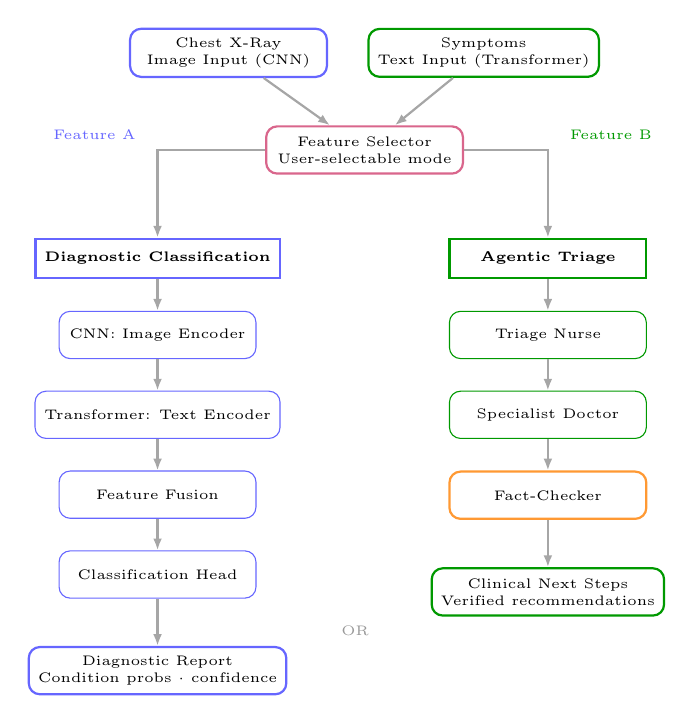
\begin{tikzpicture}[
    node distance=0.8cm and 0.5cm,
    box/.style={rectangle, draw, rounded corners, align=center, minimum width=2.5cm, minimum height=0.6cm, fill=white, font=\tiny},
    titlebox/.style={rectangle, draw, align=center, minimum width=2.5cm, minimum height=0.5cm, fill=white, font=\tiny\bfseries},
    arrow/.style={-{Latex[length=1.5mm]}, thick, draw=gray!70}
]

% 1. Inputs
\node[box, draw=blue!60, thick] (xray) {Chest X-Ray\\ Image Input (CNN)};
\node[box, draw=green!60!black, thick, right=0.5cm of xray] (symptoms) {Symptoms\\ Text Input (Transformer)};

% 2. Selector
\node[box, draw=purple!60, thick, below right=0.6cm and -0.8cm of xray] (selector) {Feature Selector\\ User-selectable mode};

% 3. Branch Headers
\node[titlebox, draw=blue!60, thick, below left=0.8cm and -0.2cm of selector] (diag_class) {Diagnostic Classification};
\node[titlebox, draw=green!60!black, thick, below right=0.8cm and -0.2cm of selector] (agentic) {Agentic Triage};

% 4. Left Branch Nodes (Feature A)
\node[box, draw=blue!60, below=0.4cm of diag_class] (cnn) {CNN: Image Encoder};
\node[box, draw=blue!60, below=0.4cm of cnn] (bilstm) {Transformer: Text Encoder};
\node[box, draw=blue!60, below=0.4cm of bilstm] (fusion) {Feature Fusion};
\node[box, draw=blue!60, below=0.4cm of fusion] (class_head) {Classification Head};

% 5. Right Branch Nodes (Feature B)
\node[box, draw=green!60!black, below=0.4cm of agentic] (nurse) {Triage Nurse};
\node[box, draw=green!60!black, below=0.4cm of nurse] (doctor) {Specialist Doctor};
\node[box, draw=orange!80, thick, below=0.4cm of doctor] (fact_checker) {Fact-Checker};

% 6. Outputs
\node[box, draw=blue!60, thick, below=0.6cm of class_head] (diag_report) {Diagnostic Report\\ Condition probs $\cdot$ confidence};
\node[box, draw=green!60!black, thick, below=0.6cm of fact_checker] (clinical_steps) {Clinical Next Steps\\ Verified recommendations};

% 7. Central "OR" text
\path (diag_report) -- (clinical_steps) node[midway, font=\tiny, color=gray!80] {OR};

% 8. Connections (Arrows)
\draw[arrow] (xray) -- (selector);
\draw[arrow] (symptoms) -- (selector);

% Path from selector to branches with labels
\draw[arrow] (selector) -| node[above, xshift=-0.8cm, font=\tiny, color=blue!60] {Feature A} (diag_class);
\draw[arrow] (selector) -| node[above, xshift=0.8cm, font=\tiny, color=green!60!black] {Feature B} (agentic);

% Left branch connections
\draw[arrow] (diag_class) -- (cnn);
\draw[arrow] (cnn) -- (bilstm);
\draw[arrow] (bilstm) -- (fusion);
\draw[arrow] (fusion) -- (class_head);
\draw[arrow] (class_head) -- (diag_report);

% Right branch connections
\draw[arrow] (agentic) -- (nurse);
\draw[arrow] (nurse) -- (doctor);
\draw[arrow] (doctor) -- (fact_checker);
\draw[arrow] (fact_checker) -- (clinical_steps);

\end{tikzpicture}
}
\caption{MediSim Model Flow detailing the dual-mode architecture: Deterministic Diagnostic Classification (Feature A) versus Generative Multi-Agent Triage (Feature B).}
\label{fig:model_flow}
\end{figure}


\section{Methodology}

\subsection{Methodological Goal and Hypotheses}
The primary objective of this project is to develop and evaluate MediSim's dual-pipeline architecture. We hypothesize that (1) a fused CNN-Transformer model will achieve higher diagnostic classification precision than isolated unimodal counterparts, and (2) our three-role multi-agent framework will produce a significantly lower hallucination rate relative to a single-agent baseline executing the same triage task.

\subsection{Datasets and Preprocessing}
To validate the Multimodal Diagnostic Assistant, we will utilize the publicly accessible IU X-Ray dataset provided via Kaggle, which comprises chest X-rays paired with clinical reports. Because the interactive Multi-Agent Triage relies on dynamic discourse, we will use synthetic patient symptomatic profiles curated from standard medical benchmarks or generated via a trusted LLM prompt pipeline to act as simulated user input. 

Preprocessing for images will involve standard rescaling, normalization, and augmentation. Textual preprocessing for the biLSTM baseline will involve tokenization, lowercasing, and removal of non-clinical stop words, eventually mapping text via GloVe or clinical Word2Vec embeddings before training.

\subsection{Models and Experimental Design}
The system bridges two primary models:
\begin{enumerate}[label=\textbf{\arabic*.}]
    \item \textbf{Vision-Language Fusion}: An ensemble approach where image features are extracted using an established CNN (e.g., ResNet18), while symptom text is embedded through a pretrained Clinical BERT Transformer network. The dense feature layers of both networks will be concatenated and fed through a classification head.
    \item \textbf{Multi-Agent Triage}: Utilizing accessible LLM APIs (e.g., Gemini 2.5 Flash via LangChain), this component initializes three distinct agents using sophisticated system prompts: the Triage Nurse, the Specialist, and the Fact-Checker. 
\end{enumerate}

\subsection{Apparatus and Compute Environment}
Experiments will be conducted on consumer-grade hardware equipped with an Apple M-series silicon or NVIDIA RTX-series GPU (min. 8GB VRAM) to ensure real-world viability. LLM interaction will be managed via high-throughput inference APIs to maintain latency below 2 seconds per turn, while local models (CNN/Transformer) will be deployed via PyTorch. The final interface will be implemented as a modern React and Firebase web application for secure, rapid cross-platform accessibility.

\subsection{Metrics}
The independent variables (IV) will be the architectural design (Unimodal vs. Multimodal fusion, and Single-Agent vs. Multi-Agent). The dependent variables (DV) will be diagnostic classification accuracy/F1-score for the fusion model, and safety/hallucination discordance rates for the triage agents.

\subsection{Training and Evaluation Protocol}
The baseline fusion model will be trained on the IU X-Ray dataset, split into 70-15-15 sets for training, validation, and testing. Performance will be monitored via loss and validated across Precision, Recall, and Accuracy. For the Generative Agent framework, quantitative evaluation will occur via human-in-the-loop clinical coherence scoring or leveraging automated metrics to compare the generated triage response against standard safe operating protocols.

\begin{table}[h]
\centering
\resizebox{\columnwidth}{!}{%
\begin{tabular}{lccccc}
\toprule
\textbf{Model} & \textbf{Acc} & \textbf{Prec} & \textbf{Rec} & \textbf{F1} & \textbf{Safety} \\
\midrule
CNN (Image Baseline) & TBD & TBD & TBD & TBD & N/A \\
\textbf{MediSim Fusion (Proposed)} & TBD & TBD & TBD & TBD & N/A \\
\midrule
Single-Agent (Triage Baseline) & - & - & - & - & Low \\
\textbf{Multi-Agent (Proposed)} & - & - & - & - & High \\
\bottomrule
\end{tabular}
}
\caption{Performance comparison between baseline architectures and the proposed MediSim components (Evaluation placeholders).}
\label{tab:performance_comparison}
\end{table}

\section{System Architecture}

The MediSim system architecture integrates a dual-pipeline approach. The first component is the Multimodal Diagnostic Assistant, which processes patient image data and textual symptom descriptions through a fused CNN and biLSTM framework. The second component is the Multi-Agent Triage system, functioning as a conversational interface powered by large language models with role-specific prompts. This unified structure ensures seamless data flow from initial patient input to final verified clinical recommendations. Additionally, the web application supports user accounts (e.g., via Firebase) to securely manage individualized API keys and retain chat history, enabling seamless continuation of diagnostic sessions and independent verification of model results.

\begin{table}[h]
\centering
\renewcommand{\arraystretch}{1.2}
\resizebox{\columnwidth}{!}{%
\begin{tabular}{l p{0.3\linewidth} p{0.4\linewidth}}
\toprule
\textbf{Feature} & \textbf{Baseline (Transformer/CNN)} & \textbf{Proposed (Multimodal + Multi-Agent)} \\
\midrule
\textbf{Modality} & Text/Image only & \textbf{Multimodal}: Text + Image \\
\textbf{Arch} & Single-stage & \textbf{Two-stage}: Vision-Lang + Agents \\
\textbf{Reasoning} & Limited & \textbf{Advanced}: Multi-agent debate \\
\textbf{Scalability} & Low & \textbf{High}: Modular agents \\
\textbf{Flexibility} & Rigid & \textbf{Versatile}: Diagnostic \& Triage \\
\textbf{Data Eff.} & High Req. & \textbf{Efficient}: Pre-trained models \\
\textbf{Error Hand.} & Single point & \textbf{Robust}: Cross-verification \\
\textbf{UX} & Static & \textbf{Interactive}: Conversational \\
\textbf{Complexity} & Low & \textbf{Medium}: Orchestration \\
\textbf{Evaluation} & BLEU/ROUGE & \textbf{Advanced}: Human + Task-specific \\
\bottomrule
\end{tabular}
}
\caption{Comparison of architectures between standard baseline models and the proposed MediSim framework.}
\label{tab:model_comparison}
\end{table}

\section{Project Timeline}

The project will be executed in four primary phases:
\begin{itemize}
    \item \textbf{Phase 1}: Literature Review and Baseline identification (Completed).
    \item \textbf{Phase 2}: Progress Report and Architecture design (Current).
    \item \textbf{Phase 3}: Implementation of the React/Firebase web application, data processing scripts, and training the baseline diagnostic models.
    \item \textbf{Phase 4}: Deployment, final evaluation, and submission.
\end{itemize}

\section{Discussion and Summary of Progress}

\subsection{Expected Discussion of Outcomes}
We anticipate that by bridging lightweight classical deep learning with modern Agentic LLM interactions, MediSim will provide accurate deterministic outputs without sacrificing dynamic patient communication. The integration of a specific Fact-Checker agent directly evaluates our core research question concerning the minimization of clinical hallucinations. If our hypothesis holds, the multi-agent system will reject unsafe responses generated by the Specialist agent, thereby maintaining high clinical coherence and directly mitigating the risks typically associated with unconstrained generative health applications. 

\subsection{Summary of Progress and Obstacles}
During Phase 1, our team successfully identified and synthesized relevant literature strictly from the ACL Anthology, identifying both our state-of-the-art inspirations and our established lightweight classification baselines. The core obstacle identified pertains to data integration: effectively matching the static image-text datasets required for the fusion model setup to the dynamic conversational structure inherently required for the multi-agent orchestration. Furthermore, maintaining execution feasibility strictly on local compute environments while juggling multiple LLM API calls may introduce latency issues, prompting our choice of rapid-inference APIs over purely local transformer hosting where necessary. Currently, all Phase 1 objectives are complete, and we are preparing to transition into code implementation and dashboard setup using a React/Firebase ecosystem.

\bibliography{references}

\end{document}
